\documentclass[twoside]{book}

% Packages required by doxygen
\usepackage{calc}
\usepackage{doxygen}
\usepackage{graphicx}
\usepackage[utf8]{inputenc}
\usepackage{makeidx}
\usepackage{multicol}
\usepackage{multirow}
\usepackage{textcomp}
\usepackage[table]{xcolor}

% Font selection
\usepackage[T1]{fontenc}
\usepackage{mathptmx}
\usepackage[scaled=.90]{helvet}
\usepackage{courier}
\usepackage{amssymb}
\usepackage{sectsty}
\renewcommand{\familydefault}{\sfdefault}
\allsectionsfont{%
  \fontseries{bc}\selectfont%
  \color{darkgray}%
}
\renewcommand{\DoxyLabelFont}{%
  \fontseries{bc}\selectfont%
  \color{darkgray}%
}

% Page & text layout
\usepackage{geometry}
\geometry{%
  a4paper,%
  top=2.5cm,%
  bottom=2.5cm,%
  left=2.5cm,%
  right=2.5cm%
}
\tolerance=750
\hfuzz=15pt
\hbadness=750
\setlength{\emergencystretch}{15pt}
\setlength{\parindent}{0cm}
\setlength{\parskip}{0.2cm}
\makeatletter
\renewcommand{\paragraph}{%
  \@startsection{paragraph}{4}{0ex}{-1.0ex}{1.0ex}{%
    \normalfont\normalsize\bfseries\SS@parafont%
  }%
}
\renewcommand{\subparagraph}{%
  \@startsection{subparagraph}{5}{0ex}{-1.0ex}{1.0ex}{%
    \normalfont\normalsize\bfseries\SS@subparafont%
  }%
}
\makeatother

% Headers & footers
\usepackage{fancyhdr}
\pagestyle{fancyplain}
\fancyhead[LE]{\fancyplain{}{\bfseries\thepage}}
\fancyhead[CE]{\fancyplain{}{}}
\fancyhead[RE]{\fancyplain{}{\bfseries\leftmark}}
\fancyhead[LO]{\fancyplain{}{\bfseries\rightmark}}
\fancyhead[CO]{\fancyplain{}{}}
\fancyhead[RO]{\fancyplain{}{\bfseries\thepage}}
\fancyfoot[LE]{\fancyplain{}{}}
\fancyfoot[CE]{\fancyplain{}{}}
\fancyfoot[RE]{\fancyplain{}{\bfseries\scriptsize Generated on Wed Apr 22 2015 12\-:54\-:56 for In\-Pace by Doxygen }}
\fancyfoot[LO]{\fancyplain{}{\bfseries\scriptsize Generated on Wed Apr 22 2015 12\-:54\-:56 for In\-Pace by Doxygen }}
\fancyfoot[CO]{\fancyplain{}{}}
\fancyfoot[RO]{\fancyplain{}{}}
\renewcommand{\footrulewidth}{0.4pt}
\renewcommand{\chaptermark}[1]{%
  \markboth{#1}{}%
}
\renewcommand{\sectionmark}[1]{%
  \markright{\thesection\ #1}%
}

% Indices & bibliography
\usepackage{natbib}
\usepackage[titles]{tocloft}
\setcounter{tocdepth}{3}
\setcounter{secnumdepth}{5}
\makeindex

% Hyperlinks (required, but should be loaded last)
\usepackage{ifpdf}
\ifpdf
  \usepackage[pdftex,pagebackref=true]{hyperref}
\else
  \usepackage[ps2pdf,pagebackref=true]{hyperref}
\fi
\hypersetup{%
  colorlinks=true,%
  linkcolor=blue,%
  citecolor=blue,%
  unicode%
}

% Custom commands
\newcommand{\clearemptydoublepage}{%
  \newpage{\pagestyle{empty}\cleardoublepage}%
}


%===== C O N T E N T S =====

\begin{document}

% Titlepage & ToC
\hypersetup{pageanchor=false}
\pagenumbering{roman}
\begin{titlepage}
\vspace*{7cm}
\begin{center}%
{\Large In\-Pace }\\
\vspace*{1cm}
{\large Generated by Doxygen 1.8.6}\\
\vspace*{0.5cm}
{\small Wed Apr 22 2015 12:54:56}\\
\end{center}
\end{titlepage}
\clearemptydoublepage
\tableofcontents
\clearemptydoublepage
\pagenumbering{arabic}
\hypersetup{pageanchor=true}

%--- Begin generated contents ---
\chapter{Hierarchical Index}
\section{Class Hierarchy}
This inheritance list is sorted roughly, but not completely, alphabetically\-:\begin{DoxyCompactList}
\item \contentsline{section}{App\-Delegate()}{\pageref{categoryAppDelegate_07_08}}{}
\item \contentsline{section}{B\-T\-Send\-Rec()}{\pageref{categoryBTSendRec_07_08}}{}
\item $<$C\-B\-Central\-Manager\-Delegate$>$\begin{DoxyCompactList}
\item \contentsline{section}{B\-T\-Discover}{\pageref{interfaceBTDiscover}}{}
\end{DoxyCompactList}
\item $<$C\-B\-Peripheral\-Delegate$>$\begin{DoxyCompactList}
\item \contentsline{section}{B\-T\-Send\-Rec}{\pageref{interfaceBTSendRec}}{}
\end{DoxyCompactList}
\item $<$C\-L\-Location\-Manager\-Delegate$>$\begin{DoxyCompactList}
\item \contentsline{section}{Route\-Info\-View\-Controller}{\pageref{interfaceRouteInfoViewController}}{}
\end{DoxyCompactList}
\item $<$M\-K\-Map\-View\-Delegate$>$\begin{DoxyCompactList}
\item \contentsline{section}{Route\-Info\-View\-Controller}{\pageref{interfaceRouteInfoViewController}}{}
\end{DoxyCompactList}
\item N\-S\-Object\begin{DoxyCompactList}
\item \contentsline{section}{B\-T\-Discover}{\pageref{interfaceBTDiscover}}{}
\item \contentsline{section}{B\-T\-Send\-Rec}{\pageref{interfaceBTSendRec}}{}
\item \contentsline{section}{Database}{\pageref{interfaceDatabase}}{}
\end{DoxyCompactList}
\item \contentsline{section}{Route\-Info\-View\-Controller()}{\pageref{categoryRouteInfoViewController_07_08}}{}
\item \contentsline{section}{Settings\-View\-Controller()}{\pageref{categorySettingsViewController_07_08}}{}
\item \contentsline{section}{Sync\-Data\-View\-Controller()}{\pageref{categorySyncDataViewController_07_08}}{}
\item $<$U\-I\-Application\-Delegate$>$\begin{DoxyCompactList}
\item \contentsline{section}{App\-Delegate}{\pageref{interfaceAppDelegate}}{}
\end{DoxyCompactList}
\item U\-I\-Responder\begin{DoxyCompactList}
\item \contentsline{section}{App\-Delegate}{\pageref{interfaceAppDelegate}}{}
\end{DoxyCompactList}
\item $<$U\-I\-Table\-View\-Data\-Source$>$\begin{DoxyCompactList}
\item \contentsline{section}{Routes\-View\-Controller}{\pageref{interfaceRoutesViewController}}{}
\item \contentsline{section}{Routes\-View\-Controller()}{\pageref{categoryRoutesViewController_07_08}}{}
\end{DoxyCompactList}
\item $<$U\-I\-Table\-View\-Delegate$>$\begin{DoxyCompactList}
\item \contentsline{section}{Routes\-View\-Controller}{\pageref{interfaceRoutesViewController}}{}
\item \contentsline{section}{Routes\-View\-Controller()}{\pageref{categoryRoutesViewController_07_08}}{}
\end{DoxyCompactList}
\item U\-I\-View\-Controller\begin{DoxyCompactList}
\item \contentsline{section}{Route\-Info\-View\-Controller}{\pageref{interfaceRouteInfoViewController}}{}
\item \contentsline{section}{Routes\-View\-Controller}{\pageref{interfaceRoutesViewController}}{}
\item \contentsline{section}{Settings\-View\-Controller}{\pageref{interfaceSettingsViewController}}{}
\item \contentsline{section}{Sync\-Data\-View\-Controller}{\pageref{interfaceSyncDataViewController}}{}
\item \contentsline{section}{View\-Controller}{\pageref{interfaceViewController}}{}
\end{DoxyCompactList}
\item \contentsline{section}{View\-Controller()}{\pageref{categoryViewController_07_08}}{}
\end{DoxyCompactList}

\chapter{Class Index}
\section{Class List}
Here are the classes, structs, unions and interfaces with brief descriptions\-:\begin{DoxyCompactList}
\item\contentsline{section}{\hyperlink{interfaceAppDelegate}{App\-Delegate} }{\pageref{interfaceAppDelegate}}{}
\item\contentsline{section}{\hyperlink{categoryAppDelegate_07_08}{App\-Delegate()} }{\pageref{categoryAppDelegate_07_08}}{}
\item\contentsline{section}{\hyperlink{interfaceBTDiscover}{B\-T\-Discover} \\*Class responsible for finding and connecting/disconnecting peripheral }{\pageref{interfaceBTDiscover}}{}
\item\contentsline{section}{\hyperlink{interfaceBTSendRec}{B\-T\-Send\-Rec} \\*Class responsible for doing the data transmission to the connected peripheral }{\pageref{interfaceBTSendRec}}{}
\item\contentsline{section}{\hyperlink{categoryBTSendRec_07_08}{B\-T\-Send\-Rec()} }{\pageref{categoryBTSendRec_07_08}}{}
\item\contentsline{section}{\hyperlink{interfaceDatabase}{Database} \\*\hyperlink{interfaceDatabase}{Database} manager class }{\pageref{interfaceDatabase}}{}
\item\contentsline{section}{\hyperlink{interfaceRouteInfoViewController}{Route\-Info\-View\-Controller} }{\pageref{interfaceRouteInfoViewController}}{}
\item\contentsline{section}{\hyperlink{categoryRouteInfoViewController_07_08}{Route\-Info\-View\-Controller()} }{\pageref{categoryRouteInfoViewController_07_08}}{}
\item\contentsline{section}{\hyperlink{interfaceRoutesViewController}{Routes\-View\-Controller} }{\pageref{interfaceRoutesViewController}}{}
\item\contentsline{section}{\hyperlink{categoryRoutesViewController_07_08}{Routes\-View\-Controller()} }{\pageref{categoryRoutesViewController_07_08}}{}
\item\contentsline{section}{\hyperlink{interfaceSettingsViewController}{Settings\-View\-Controller} }{\pageref{interfaceSettingsViewController}}{}
\item\contentsline{section}{\hyperlink{categorySettingsViewController_07_08}{Settings\-View\-Controller()} }{\pageref{categorySettingsViewController_07_08}}{}
\item\contentsline{section}{\hyperlink{interfaceSyncDataViewController}{Sync\-Data\-View\-Controller} }{\pageref{interfaceSyncDataViewController}}{}
\item\contentsline{section}{\hyperlink{categorySyncDataViewController_07_08}{Sync\-Data\-View\-Controller()} }{\pageref{categorySyncDataViewController_07_08}}{}
\item\contentsline{section}{\hyperlink{interfaceViewController}{View\-Controller} }{\pageref{interfaceViewController}}{}
\item\contentsline{section}{\hyperlink{categoryViewController_07_08}{View\-Controller()} }{\pageref{categoryViewController_07_08}}{}
\end{DoxyCompactList}

\chapter{File Index}
\section{File List}
Here is a list of all documented files with brief descriptions\-:\begin{DoxyCompactList}
\item\contentsline{section}{In\-Pace/\-In\-Pace/{\bfseries App\-Delegate.\-h} }{\pageref{AppDelegate_8h}}{}
\item\contentsline{section}{In\-Pace/\-In\-Pace/{\bfseries B\-T\-Discover.\-h} }{\pageref{BTDiscover_8h}}{}
\item\contentsline{section}{In\-Pace/\-In\-Pace/\hyperlink{BTSendRec_8h}{B\-T\-Send\-Rec.\-h} \\*Bluetooth send and receive functionality }{\pageref{BTSendRec_8h}}{}
\item\contentsline{section}{In\-Pace/\-In\-Pace/{\bfseries Database.\-h} }{\pageref{Database_8h}}{}
\item\contentsline{section}{In\-Pace/\-In\-Pace/{\bfseries Route\-Info\-View\-Controller.\-h} }{\pageref{RouteInfoViewController_8h}}{}
\item\contentsline{section}{In\-Pace/\-In\-Pace/{\bfseries Routes\-View\-Controller.\-h} }{\pageref{RoutesViewController_8h}}{}
\item\contentsline{section}{In\-Pace/\-In\-Pace/{\bfseries Settings\-View\-Controller.\-h} }{\pageref{SettingsViewController_8h}}{}
\item\contentsline{section}{In\-Pace/\-In\-Pace/{\bfseries Sync\-Data\-View\-Controller.\-h} }{\pageref{SyncDataViewController_8h}}{}
\item\contentsline{section}{In\-Pace/\-In\-Pace/{\bfseries View\-Controller.\-h} }{\pageref{ViewController_8h}}{}
\end{DoxyCompactList}

\chapter{Class Documentation}
\hypertarget{interfaceAppDelegate}{\section{App\-Delegate Class Reference}
\label{interfaceAppDelegate}\index{App\-Delegate@{App\-Delegate}}
}
Inheritance diagram for App\-Delegate\-:\begin{figure}[H]
\begin{center}
\leavevmode
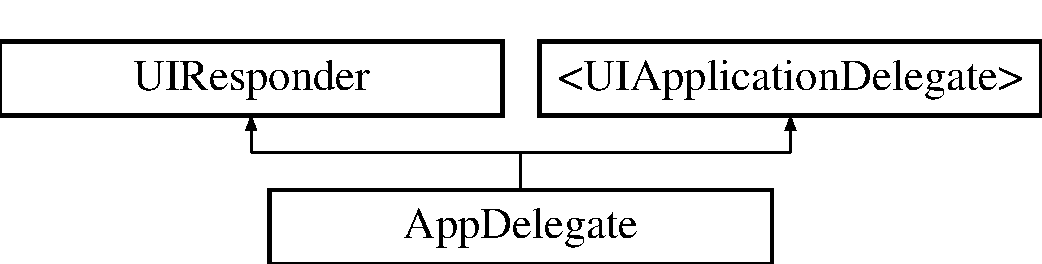
\includegraphics[height=2.000000cm]{interfaceAppDelegate}
\end{center}
\end{figure}


The documentation for this class was generated from the following file\-:\begin{DoxyCompactItemize}
\item 
In\-Pace/\-In\-Pace/App\-Delegate.\-h\end{DoxyCompactItemize}

\hypertarget{categoryAppDelegate_07_08}{\section{App\-Delegate() Category Reference}
\label{categoryAppDelegate_07_08}\index{App\-Delegate()@{App\-Delegate()}}
}


The documentation for this category was generated from the following file\-:\begin{DoxyCompactItemize}
\item 
In\-Pace/\-In\-Pace/App\-Delegate.\-m\end{DoxyCompactItemize}

\hypertarget{interfaceBTDiscover}{\section{B\-T\-Discover Class Reference}
\label{interfaceBTDiscover}\index{B\-T\-Discover@{B\-T\-Discover}}
}


Class responsible for finding and connecting/disconnecting peripheral.  




{\ttfamily \#import $<$B\-T\-Discover.\-h$>$}

Inheritance diagram for B\-T\-Discover\-:\begin{figure}[H]
\begin{center}
\leavevmode
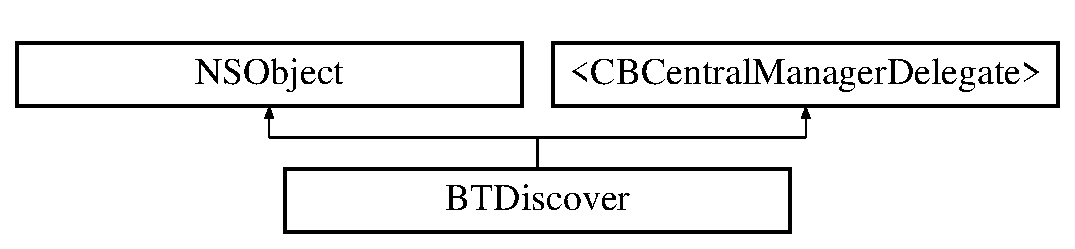
\includegraphics[height=2.000000cm]{interfaceBTDiscover}
\end{center}
\end{figure}
\subsection*{Instance Methods}
\begin{DoxyCompactItemize}
\item 
(void) -\/ \hyperlink{interfaceBTDiscover_a8f79744b7fda346637a523075043b501}{scan\-For\-Wristband}
\item 
(void) -\/ \hyperlink{interfaceBTDiscover_aee431dcb8f6de0bbaa3b812e8e48cdbc}{central\-Manager\-Did\-Update\-State\-:}
\item 
(void) -\/ \hyperlink{interfaceBTDiscover_af8e43de53c115f15bff0eeccbcdf260a}{central\-Manager\-:did\-Discover\-Peripheral\-:advertisement\-Data\-:\-R\-S\-S\-I\-:}
\item 
(void) -\/ \hyperlink{interfaceBTDiscover_a892d491ba386390b6f774c141e278054}{central\-Manager\-:did\-Connect\-Peripheral\-:}
\item 
(void) -\/ \hyperlink{interfaceBTDiscover_a97b8fd0dd542e6b41378922977ecbb0d}{central\-Manager\-:did\-Disconnect\-Peripheral\-:error\-:}
\end{DoxyCompactItemize}
\subsection*{Properties}
\begin{DoxyCompactItemize}
\item 
\hyperlink{interfaceBTSendRec}{B\-T\-Send\-Rec} $\ast$ \hyperlink{interfaceBTDiscover_ac6fc7e50655c8ad721cb1e3a167767b6}{wristband}
\item 
C\-B\-Central\-Manager $\ast$ \hyperlink{interfaceBTDiscover_a7e656419213fe4da7163a7fc82fcc2a9}{manager}
\item 
C\-B\-Peripheral $\ast$ \hyperlink{interfaceBTDiscover_a611f96cb207ccfc4bc06e33f54183374}{bt\-\_\-periph}
\end{DoxyCompactItemize}


\subsection{Detailed Description}
Class responsible for finding and connecting/disconnecting peripheral. 

This class is largely a wrapper around the C\-B\-Central\-Manager class and also acts as its delegate object. As such, many of its functions are implemented so the class conforms to the \hyperlink{classCBCentralManagerDelegate-p}{C\-B\-Central\-Manager\-Delegate} protocol. 

\subsection{Method Documentation}
\hypertarget{interfaceBTDiscover_a892d491ba386390b6f774c141e278054}{\index{B\-T\-Discover@{B\-T\-Discover}!central\-Manager\-:did\-Connect\-Peripheral\-:@{central\-Manager\-:did\-Connect\-Peripheral\-:}}
\index{central\-Manager\-:did\-Connect\-Peripheral\-:@{central\-Manager\-:did\-Connect\-Peripheral\-:}!BTDiscover@{B\-T\-Discover}}
\subsubsection[{central\-Manager\-:did\-Connect\-Peripheral\-:}]{\setlength{\rightskip}{0pt plus 5cm}-\/ (void) central\-Manager\-: 
\begin{DoxyParamCaption}
\item[{(C\-B\-Central\-Manager$\ast$)}]{central}
\item[{didConnectPeripheral:(C\-B\-Peripheral$\ast$)}]{peripheral}
\end{DoxyParamCaption}
}}\label{interfaceBTDiscover_a892d491ba386390b6f774c141e278054}
This function is called when a peripheral was successfully connected to by our C\-B\-Central\-Manager object. Part of the C\-B\-Central\-Manager\-Delegate\-Protocol. 
\begin{DoxyParams}{Parameters}
{\em central} & The C\-B\-Central\-Manager object \\
\hline
{\em peripheral} & The peripheral that just got connected \\
\hline
\end{DoxyParams}
\hypertarget{interfaceBTDiscover_a97b8fd0dd542e6b41378922977ecbb0d}{\index{B\-T\-Discover@{B\-T\-Discover}!central\-Manager\-:did\-Disconnect\-Peripheral\-:error\-:@{central\-Manager\-:did\-Disconnect\-Peripheral\-:error\-:}}
\index{central\-Manager\-:did\-Disconnect\-Peripheral\-:error\-:@{central\-Manager\-:did\-Disconnect\-Peripheral\-:error\-:}!BTDiscover@{B\-T\-Discover}}
\subsubsection[{central\-Manager\-:did\-Disconnect\-Peripheral\-:error\-:}]{\setlength{\rightskip}{0pt plus 5cm}-\/ (void) central\-Manager\-: 
\begin{DoxyParamCaption}
\item[{(C\-B\-Central\-Manager$\ast$)}]{central}
\item[{didDisconnectPeripheral:(C\-B\-Peripheral$\ast$)}]{peripheral}
\item[{error:(N\-S\-Error$\ast$)}]{error}
\end{DoxyParamCaption}
}}\label{interfaceBTDiscover_a97b8fd0dd542e6b41378922977ecbb0d}
This function is called when a peripheral has disconnected. Part of the \hyperlink{classCBCentralManagerDelegate-p}{C\-B\-Central\-Manager\-Delegate} protocol. 
\begin{DoxyParams}{Parameters}
{\em central} & The central manager object \\
\hline
{\em peripheral} & The peripheral that has been disconnected \\
\hline
{\em error} & The cause of faliure, if any \\
\hline
\end{DoxyParams}
\hypertarget{interfaceBTDiscover_af8e43de53c115f15bff0eeccbcdf260a}{\index{B\-T\-Discover@{B\-T\-Discover}!central\-Manager\-:did\-Discover\-Peripheral\-:advertisement\-Data\-:\-R\-S\-S\-I\-:@{central\-Manager\-:did\-Discover\-Peripheral\-:advertisement\-Data\-:\-R\-S\-S\-I\-:}}
\index{central\-Manager\-:did\-Discover\-Peripheral\-:advertisement\-Data\-:\-R\-S\-S\-I\-:@{central\-Manager\-:did\-Discover\-Peripheral\-:advertisement\-Data\-:\-R\-S\-S\-I\-:}!BTDiscover@{B\-T\-Discover}}
\subsubsection[{central\-Manager\-:did\-Discover\-Peripheral\-:advertisement\-Data\-:\-R\-S\-S\-I\-:}]{\setlength{\rightskip}{0pt plus 5cm}-\/ (void) central\-Manager\-: 
\begin{DoxyParamCaption}
\item[{(C\-B\-Central\-Manager$\ast$)}]{central}
\item[{didDiscoverPeripheral:(C\-B\-Peripheral$\ast$)}]{peripheral}
\item[{advertisementData:(N\-S\-Dictionary$\ast$)}]{advertisement\-Data}
\item[{RSSI:(N\-S\-Number$\ast$)}]{R\-S\-S\-I}
\end{DoxyParamCaption}
}}\label{interfaceBTDiscover_af8e43de53c115f15bff0eeccbcdf260a}
This function is called when a peripheral was discovered during scanning by the C\-B\-Central\-Manager object. Part of the \hyperlink{classCBCentralManagerDelegate-p}{C\-B\-Central\-Manager\-Delegate} protocol. 
\begin{DoxyParams}{Parameters}
{\em central} & The central manager object \\
\hline
{\em peripheral} & The discovered peripheral \\
\hline
{\em advertisement\-Data} & The advertisement data (if any) \\
\hline
{\em R\-S\-S\-I} & The signal strength \\
\hline
\end{DoxyParams}
\hypertarget{interfaceBTDiscover_aee431dcb8f6de0bbaa3b812e8e48cdbc}{\index{B\-T\-Discover@{B\-T\-Discover}!central\-Manager\-Did\-Update\-State\-:@{central\-Manager\-Did\-Update\-State\-:}}
\index{central\-Manager\-Did\-Update\-State\-:@{central\-Manager\-Did\-Update\-State\-:}!BTDiscover@{B\-T\-Discover}}
\subsubsection[{central\-Manager\-Did\-Update\-State\-:}]{\setlength{\rightskip}{0pt plus 5cm}-\/ (void) central\-Manager\-Did\-Update\-State\-: 
\begin{DoxyParamCaption}
\item[{(C\-B\-Central\-Manager$\ast$)}]{central}
\end{DoxyParamCaption}
}}\label{interfaceBTDiscover_aee431dcb8f6de0bbaa3b812e8e48cdbc}
This function is called whenever the C\-B\-Central\-Manager object changes its state. This function is required by the \hyperlink{classCBCentralManagerDelegate-p}{C\-B\-Central\-Manager\-Delegate} protocol. 
\begin{DoxyParams}{Parameters}
{\em central} & The central manager object \\
\hline
\end{DoxyParams}
\hypertarget{interfaceBTDiscover_a8f79744b7fda346637a523075043b501}{\index{B\-T\-Discover@{B\-T\-Discover}!scan\-For\-Wristband@{scan\-For\-Wristband}}
\index{scan\-For\-Wristband@{scan\-For\-Wristband}!BTDiscover@{B\-T\-Discover}}
\subsubsection[{scan\-For\-Wristband}]{\setlength{\rightskip}{0pt plus 5cm}-\/ (void) scan\-For\-Wristband 
\begin{DoxyParamCaption}
{}
\end{DoxyParamCaption}
}}\label{interfaceBTDiscover_a8f79744b7fda346637a523075043b501}
Initiate scan for the In\-Pace wristband 

\subsection{Property Documentation}
\hypertarget{interfaceBTDiscover_a611f96cb207ccfc4bc06e33f54183374}{\index{B\-T\-Discover@{B\-T\-Discover}!bt\-\_\-periph@{bt\-\_\-periph}}
\index{bt\-\_\-periph@{bt\-\_\-periph}!BTDiscover@{B\-T\-Discover}}
\subsubsection[{bt\-\_\-periph}]{\setlength{\rightskip}{0pt plus 5cm}-\/ (C\-B\-Peripheral$\ast$) bt\-\_\-periph\hspace{0.3cm}{\ttfamily [read]}, {\ttfamily [write]}, {\ttfamily [atomic]}, {\ttfamily [strong]}}}\label{interfaceBTDiscover_a611f96cb207ccfc4bc06e33f54183374}
Pointer to the discovered Bluetooth peripheral \hypertarget{interfaceBTDiscover_a7e656419213fe4da7163a7fc82fcc2a9}{\index{B\-T\-Discover@{B\-T\-Discover}!manager@{manager}}
\index{manager@{manager}!BTDiscover@{B\-T\-Discover}}
\subsubsection[{manager}]{\setlength{\rightskip}{0pt plus 5cm}-\/ (C\-B\-Central\-Manager$\ast$) manager\hspace{0.3cm}{\ttfamily [read]}, {\ttfamily [write]}, {\ttfamily [atomic]}, {\ttfamily [strong]}}}\label{interfaceBTDiscover_a7e656419213fe4da7163a7fc82fcc2a9}
Pointer to the internal central manager object \hypertarget{interfaceBTDiscover_ac6fc7e50655c8ad721cb1e3a167767b6}{\index{B\-T\-Discover@{B\-T\-Discover}!wristband@{wristband}}
\index{wristband@{wristband}!BTDiscover@{B\-T\-Discover}}
\subsubsection[{wristband}]{\setlength{\rightskip}{0pt plus 5cm}-\/ ({\bf B\-T\-Send\-Rec}$\ast$) wristband\hspace{0.3cm}{\ttfamily [read]}, {\ttfamily [write]}, {\ttfamily [nonatomic]}, {\ttfamily [strong]}}}\label{interfaceBTDiscover_ac6fc7e50655c8ad721cb1e3a167767b6}
Pointer to class to handle sending and receiving data to and from the Bluetooth peripheral 

The documentation for this class was generated from the following files\-:\begin{DoxyCompactItemize}
\item 
In\-Pace/\-In\-Pace/B\-T\-Discover.\-h\item 
In\-Pace/\-In\-Pace/B\-T\-Discover.\-m\end{DoxyCompactItemize}

\hypertarget{interfaceBTSendRec}{\section{B\-T\-Send\-Rec Class Reference}
\label{interfaceBTSendRec}\index{B\-T\-Send\-Rec@{B\-T\-Send\-Rec}}
}


Class responsible for doing the data transmission to the connected peripheral.  




{\ttfamily \#import $<$B\-T\-Send\-Rec.\-h$>$}

Inheritance diagram for B\-T\-Send\-Rec\-:\begin{figure}[H]
\begin{center}
\leavevmode
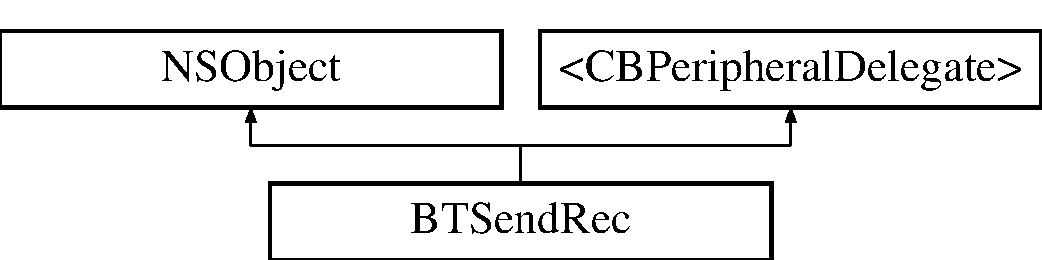
\includegraphics[height=2.000000cm]{interfaceBTSendRec}
\end{center}
\end{figure}
\subsection*{Instance Methods}
\begin{DoxyCompactItemize}
\item 
(void) -\/ \hyperlink{interfaceBTSendRec_ac2435c7aa9df21d6d3ffc2b570c15fb7}{write\-File\-:to\-Database\-:}
\item 
(double) -\/ \hyperlink{interfaceBTSendRec_afebf4e21bbbc80a1fdd04f1d5920d258}{distance\-:second\-Point\-:}
\item 
(int) -\/ \hyperlink{interfaceBTSendRec_a2c40741a15aca7b2fae51be9e469ccd8}{time\-:end\-Time\-:}
\end{DoxyCompactItemize}


\subsection{Detailed Description}
Class responsible for doing the data transmission to the connected peripheral. 

This class is largely a wrapper around C\-B\-Peripheral and also acts as its delegate object. As such, many functions are implemented so the class conforms to the \hyperlink{classCBPeripheralDelegate-p}{C\-B\-Peripheral\-Delegate} protocol. 

\subsection{Method Documentation}
\hypertarget{interfaceBTSendRec_afebf4e21bbbc80a1fdd04f1d5920d258}{\index{B\-T\-Send\-Rec@{B\-T\-Send\-Rec}!distance\-:second\-Point\-:@{distance\-:second\-Point\-:}}
\index{distance\-:second\-Point\-:@{distance\-:second\-Point\-:}!BTSendRec@{B\-T\-Send\-Rec}}
\subsubsection[{distance\-:second\-Point\-:}]{\setlength{\rightskip}{0pt plus 5cm}-\/ (double) distance\-: 
\begin{DoxyParamCaption}
\item[{(double$\ast$)}]{p1}
\item[{secondPoint:(double$\ast$)}]{p2}
\end{DoxyParamCaption}
}}\label{interfaceBTSendRec_afebf4e21bbbc80a1fdd04f1d5920d258}
This function uses the Haversine Formula to compute the distance between two pairs of G\-P\-S coordinates. Both input parameters are assumed to be arrays of doubles of the form \mbox{[}Latitude, Longitude\mbox{]}, both of which are in degrees. 
\begin{DoxyParams}{Parameters}
{\em p1} & An array of doubles of size 2 containing a pair of G\-P\-S coordinates \\
\hline
{\em p2} & An array of doubles of size 2 containing a pair of G\-P\-S coordinates \\
\hline
\end{DoxyParams}
\begin{DoxyReturn}{Returns}
The function returns the calculated distance between the two points 
\end{DoxyReturn}
\hypertarget{interfaceBTSendRec_a2c40741a15aca7b2fae51be9e469ccd8}{\index{B\-T\-Send\-Rec@{B\-T\-Send\-Rec}!time\-:end\-Time\-:@{time\-:end\-Time\-:}}
\index{time\-:end\-Time\-:@{time\-:end\-Time\-:}!BTSendRec@{B\-T\-Send\-Rec}}
\subsubsection[{time\-:end\-Time\-:}]{\setlength{\rightskip}{0pt plus 5cm}-\/ (int) time\-: 
\begin{DoxyParamCaption}
\item[{(int$\ast$)}]{start}
\item[{endTime:(int$\ast$)}]{end}
\end{DoxyParamCaption}
}}\label{interfaceBTSendRec_a2c40741a15aca7b2fae51be9e469ccd8}
This function computes the difference between two timestamps. Both paramaters are assumed to be arrays of doubles of the form \mbox{[}Year, Month, Day, Hour, Minute, Second\mbox{]}. 
\begin{DoxyParams}{Parameters}
{\em start} & An array of ints of size 6 containing time information \\
\hline
{\em end} & An array of ints of size 6 containing time information \\
\hline
\end{DoxyParams}
\begin{DoxyReturn}{Returns}
The function returns the difference bewtween the two times in seconds 
\end{DoxyReturn}
\hypertarget{interfaceBTSendRec_ac2435c7aa9df21d6d3ffc2b570c15fb7}{\index{B\-T\-Send\-Rec@{B\-T\-Send\-Rec}!write\-File\-:to\-Database\-:@{write\-File\-:to\-Database\-:}}
\index{write\-File\-:to\-Database\-:@{write\-File\-:to\-Database\-:}!BTSendRec@{B\-T\-Send\-Rec}}
\subsubsection[{write\-File\-:to\-Database\-:}]{\setlength{\rightskip}{0pt plus 5cm}-\/ (void) write\-File\-: 
\begin{DoxyParamCaption}
\item[{(N\-S\-String$\ast$)}]{filename}
\item[{toDatabase:({\bf Database}$\ast$)}]{db}
\end{DoxyParamCaption}
}}\label{interfaceBTSendRec_ac2435c7aa9df21d6d3ffc2b570c15fb7}

\begin{DoxyParams}{Parameters}
{\em filename} & The name of the file whose content is to be parsed and placed into a database \\
\hline
{\em db} & The database where the data will be stored \\
\hline
\end{DoxyParams}


The documentation for this class was generated from the following files\-:\begin{DoxyCompactItemize}
\item 
In\-Pace/\-In\-Pace/\hyperlink{BTSendRec_8h}{B\-T\-Send\-Rec.\-h}\item 
In\-Pace/\-In\-Pace/B\-T\-Send\-Rec.\-m\end{DoxyCompactItemize}

\hypertarget{categoryBTSendRec_07_08}{\section{B\-T\-Send\-Rec() Category Reference}
\label{categoryBTSendRec_07_08}\index{B\-T\-Send\-Rec()@{B\-T\-Send\-Rec()}}
}


The documentation for this category was generated from the following file\-:\begin{DoxyCompactItemize}
\item 
In\-Pace/\-In\-Pace/B\-T\-Send\-Rec.\-m\end{DoxyCompactItemize}

\hypertarget{interfaceDatabase}{\section{Database Class Reference}
\label{interfaceDatabase}\index{Database@{Database}}
}


\hyperlink{interfaceDatabase}{Database} manager class.  




{\ttfamily \#import $<$Database.\-h$>$}

Inheritance diagram for Database\-:\begin{figure}[H]
\begin{center}
\leavevmode
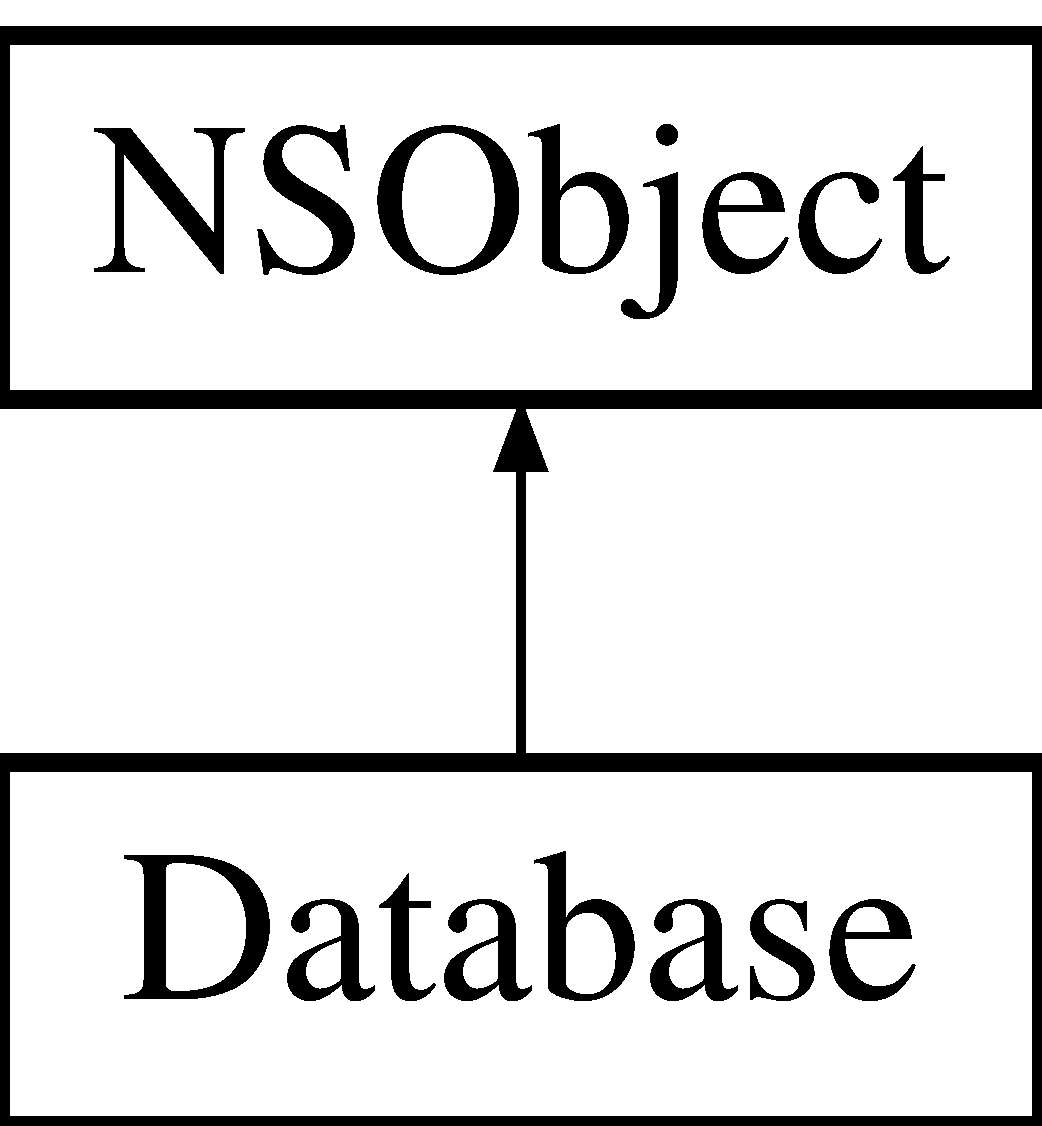
\includegraphics[height=2.000000cm]{interfaceDatabase}
\end{center}
\end{figure}
\subsection*{Instance Methods}
\begin{DoxyCompactItemize}
\item 
(instancetype) -\/ \hyperlink{interfaceDatabase_a631bb1f508de7a8397e51319c7d81100}{init\-\_\-dbfile\-:}
\item 
(int) -\/ \hyperlink{interfaceDatabase_a5cee36b8ec7d12bb7c43fc3c2581d848}{query\-:}
\end{DoxyCompactItemize}
\subsection*{Properties}
\begin{DoxyCompactItemize}
\item 
N\-S\-String $\ast$ \hyperlink{interfaceDatabase_a430fb12f30886311e10ce028918c11fa}{file}
\item 
N\-S\-Mutable\-Array $\ast$ \hyperlink{interfaceDatabase_aaf90264ccd741532c3b9258a82faa921}{results}
\item 
N\-S\-Mutable\-Array $\ast$ \hyperlink{interfaceDatabase_a1bd01161d2f5a26a74edccc2288b5774}{columns}
\item 
long long int \hyperlink{interfaceDatabase_ac733c637b2bf08cae3005686867338f9}{last\-\_\-rowid}
\end{DoxyCompactItemize}


\subsection{Detailed Description}
\hyperlink{interfaceDatabase}{Database} manager class. 

This class maintains an S\-Q\-L\-I\-T\-E database to hold the various Routes, Coordinates, and Times. 

\subsection{Method Documentation}
\hypertarget{interfaceDatabase_a631bb1f508de7a8397e51319c7d81100}{\index{Database@{Database}!init\-\_\-dbfile\-:@{init\-\_\-dbfile\-:}}
\index{init\-\_\-dbfile\-:@{init\-\_\-dbfile\-:}!Database@{Database}}
\subsubsection[{init\-\_\-dbfile\-:}]{\setlength{\rightskip}{0pt plus 5cm}-\/ (instancetype) init\-\_\-dbfile\-: 
\begin{DoxyParamCaption}
\item[{(N\-S\-String$\ast$)}]{filename}
\end{DoxyParamCaption}
}}\label{interfaceDatabase_a631bb1f508de7a8397e51319c7d81100}
Initialization function for the \hyperlink{interfaceDatabase}{Database} object. The \hyperlink{interfaceDatabase}{Database} will use the file given by filename to store and load its data. 
\begin{DoxyParams}{Parameters}
{\em filename} & The name of the file to use as the database file \\
\hline
\end{DoxyParams}
\begin{DoxyReturn}{Returns}
A pointer to the newly created \hyperlink{interfaceDatabase}{Database} object is returned 
\end{DoxyReturn}
\hypertarget{interfaceDatabase_a5cee36b8ec7d12bb7c43fc3c2581d848}{\index{Database@{Database}!query\-:@{query\-:}}
\index{query\-:@{query\-:}!Database@{Database}}
\subsubsection[{query\-:}]{\setlength{\rightskip}{0pt plus 5cm}-\/ (int) query\-: 
\begin{DoxyParamCaption}
\item[{(N\-S\-String$\ast$)}]{query}
\end{DoxyParamCaption}
}}\label{interfaceDatabase_a5cee36b8ec7d12bb7c43fc3c2581d848}
The main function of the database. This function takes an S\-Q\-L statement given by query and executes it on the database. If the satement executed was a S\-E\-L\-E\-C\-T statement, then the results will be stored in the arrays results and columns. Any other statement will simply results in these two arrays being empty. query() returns a status code from the S\-Q\-L\-I\-T\-E3 library to indicate the the success of the statement. 
\begin{DoxyParams}{Parameters}
{\em query} & The desired S\-Q\-L\-I\-T\-E statement to be executed \\
\hline
\end{DoxyParams}
\begin{DoxyReturn}{Returns}
An S\-Q\-L\-I\-T\-E3 result code indicating the status of the statement 
\end{DoxyReturn}


\subsection{Property Documentation}
\hypertarget{interfaceDatabase_a1bd01161d2f5a26a74edccc2288b5774}{\index{Database@{Database}!columns@{columns}}
\index{columns@{columns}!Database@{Database}}
\subsubsection[{columns}]{\setlength{\rightskip}{0pt plus 5cm}-\/ (N\-S\-Mutable\-Array$\ast$) columns\hspace{0.3cm}{\ttfamily [read]}, {\ttfamily [write]}, {\ttfamily [atomic]}, {\ttfamily [retain]}}}\label{interfaceDatabase_a1bd01161d2f5a26a74edccc2288b5774}
Array to hold names of columns in result \hypertarget{interfaceDatabase_a430fb12f30886311e10ce028918c11fa}{\index{Database@{Database}!file@{file}}
\index{file@{file}!Database@{Database}}
\subsubsection[{file}]{\setlength{\rightskip}{0pt plus 5cm}-\/ (N\-S\-String$\ast$) file\hspace{0.3cm}{\ttfamily [read]}, {\ttfamily [write]}, {\ttfamily [atomic]}, {\ttfamily [retain]}}}\label{interfaceDatabase_a430fb12f30886311e10ce028918c11fa}
Name of database file \hypertarget{interfaceDatabase_ac733c637b2bf08cae3005686867338f9}{\index{Database@{Database}!last\-\_\-rowid@{last\-\_\-rowid}}
\index{last\-\_\-rowid@{last\-\_\-rowid}!Database@{Database}}
\subsubsection[{last\-\_\-rowid}]{\setlength{\rightskip}{0pt plus 5cm}-\/ (long long int) last\-\_\-rowid\hspace{0.3cm}{\ttfamily [read]}, {\ttfamily [write]}, {\ttfamily [atomic]}, {\ttfamily [assign]}}}\label{interfaceDatabase_ac733c637b2bf08cae3005686867338f9}
Row\-I\-D of the last thing inserted into the database \hypertarget{interfaceDatabase_aaf90264ccd741532c3b9258a82faa921}{\index{Database@{Database}!results@{results}}
\index{results@{results}!Database@{Database}}
\subsubsection[{results}]{\setlength{\rightskip}{0pt plus 5cm}-\/ (N\-S\-Mutable\-Array$\ast$) results\hspace{0.3cm}{\ttfamily [read]}, {\ttfamily [write]}, {\ttfamily [atomic]}, {\ttfamily [retain]}}}\label{interfaceDatabase_aaf90264ccd741532c3b9258a82faa921}
Array to hold query results 

The documentation for this class was generated from the following files\-:\begin{DoxyCompactItemize}
\item 
In\-Pace/\-In\-Pace/Database.\-h\item 
In\-Pace/\-In\-Pace/Database.\-m\end{DoxyCompactItemize}

\hypertarget{interfaceRouteInfoViewController}{\section{Route\-Info\-View\-Controller Class Reference}
\label{interfaceRouteInfoViewController}\index{Route\-Info\-View\-Controller@{Route\-Info\-View\-Controller}}
}


{\ttfamily \#import $<$Route\-Info\-View\-Controller.\-h$>$}

Inheritance diagram for Route\-Info\-View\-Controller\-:\begin{figure}[H]
\begin{center}
\leavevmode
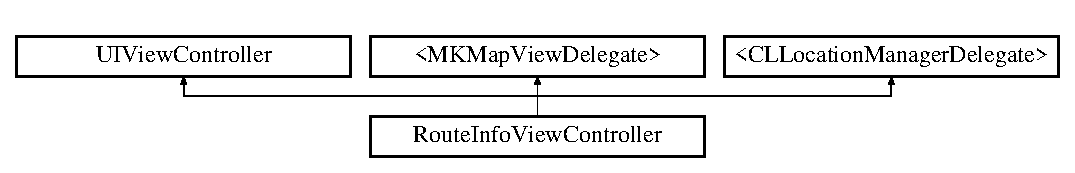
\includegraphics[height=1.876047cm]{interfaceRouteInfoViewController}
\end{center}
\end{figure}
\subsection*{Instance Methods}
\begin{DoxyCompactItemize}
\item 
(void) -\/ \hyperlink{interfaceRouteInfoViewController_a8bfec5ad745b6192124fc9dab10775a8}{load\-Route\-Data}
\end{DoxyCompactItemize}
\subsection*{Properties}
\begin{DoxyCompactItemize}
\item 
I\-B\-Outlet M\-K\-Map\-View $\ast$ \hyperlink{interfaceRouteInfoViewController_a05fec55f48777eed52aea7872128648b}{map\-View}
\item 
long long int \hyperlink{interfaceRouteInfoViewController_ada165232dfcc705567763b8b5ad234c1}{route\-I\-D}
\item 
\hyperlink{interfaceDatabase}{Database} $\ast$ \hyperlink{interfaceRouteInfoViewController_abca6639d927411ab6d56c47859f42d85}{db\-Manager}
\item 
N\-S\-Mutable\-Array $\ast$ \hyperlink{interfaceRouteInfoViewController_a4f2d1dc4014af950cfad38306ca87d0e}{arr\-Route\-Coord}
\end{DoxyCompactItemize}


\subsection{Detailed Description}
\hyperlink{interfaceViewController}{View\-Controller} for viewing map and graph representation of individual route data 

\subsection{Method Documentation}
\hypertarget{interfaceRouteInfoViewController_a8bfec5ad745b6192124fc9dab10775a8}{\index{Route\-Info\-View\-Controller@{Route\-Info\-View\-Controller}!load\-Route\-Data@{load\-Route\-Data}}
\index{load\-Route\-Data@{load\-Route\-Data}!RouteInfoViewController@{Route\-Info\-View\-Controller}}
\subsubsection[{load\-Route\-Data}]{\setlength{\rightskip}{0pt plus 5cm}-\/ (void) load\-Route\-Data 
\begin{DoxyParamCaption}
{}
\end{DoxyParamCaption}
}}\label{interfaceRouteInfoViewController_a8bfec5ad745b6192124fc9dab10775a8}
Method for pulling individual route coordinates based on the route\-I\-D 

\subsection{Property Documentation}
\hypertarget{interfaceRouteInfoViewController_a4f2d1dc4014af950cfad38306ca87d0e}{\index{Route\-Info\-View\-Controller@{Route\-Info\-View\-Controller}!arr\-Route\-Coord@{arr\-Route\-Coord}}
\index{arr\-Route\-Coord@{arr\-Route\-Coord}!RouteInfoViewController@{Route\-Info\-View\-Controller}}
\subsubsection[{arr\-Route\-Coord}]{\setlength{\rightskip}{0pt plus 5cm}-\/ (N\-S\-Mutable\-Array$\ast$) arr\-Route\-Coord\hspace{0.3cm}{\ttfamily [read]}, {\ttfamily [write]}, {\ttfamily [nonatomic]}, {\ttfamily [strong]}}}\label{interfaceRouteInfoViewController_a4f2d1dc4014af950cfad38306ca87d0e}
array for holding route coordinates from D\-B \hypertarget{interfaceRouteInfoViewController_abca6639d927411ab6d56c47859f42d85}{\index{Route\-Info\-View\-Controller@{Route\-Info\-View\-Controller}!db\-Manager@{db\-Manager}}
\index{db\-Manager@{db\-Manager}!RouteInfoViewController@{Route\-Info\-View\-Controller}}
\subsubsection[{db\-Manager}]{\setlength{\rightskip}{0pt plus 5cm}-\/ ({\bf Database}$\ast$) db\-Manager\hspace{0.3cm}{\ttfamily [read]}, {\ttfamily [write]}, {\ttfamily [nonatomic]}, {\ttfamily [strong]}}}\label{interfaceRouteInfoViewController_abca6639d927411ab6d56c47859f42d85}
instance of \hyperlink{interfaceDatabase}{Database} \hypertarget{interfaceRouteInfoViewController_a05fec55f48777eed52aea7872128648b}{\index{Route\-Info\-View\-Controller@{Route\-Info\-View\-Controller}!map\-View@{map\-View}}
\index{map\-View@{map\-View}!RouteInfoViewController@{Route\-Info\-View\-Controller}}
\subsubsection[{map\-View}]{\setlength{\rightskip}{0pt plus 5cm}-\/ (I\-B\-Outlet M\-K\-Map\-View$\ast$) map\-View\hspace{0.3cm}{\ttfamily [read]}, {\ttfamily [write]}, {\ttfamily [nonatomic]}, {\ttfamily [retain]}}}\label{interfaceRouteInfoViewController_a05fec55f48777eed52aea7872128648b}
Map View \hypertarget{interfaceRouteInfoViewController_ada165232dfcc705567763b8b5ad234c1}{\index{Route\-Info\-View\-Controller@{Route\-Info\-View\-Controller}!route\-I\-D@{route\-I\-D}}
\index{route\-I\-D@{route\-I\-D}!RouteInfoViewController@{Route\-Info\-View\-Controller}}
\subsubsection[{route\-I\-D}]{\setlength{\rightskip}{0pt plus 5cm}-\/ (long long int) route\-I\-D\hspace{0.3cm}{\ttfamily [read]}, {\ttfamily [write]}, {\ttfamily [nonatomic]}, {\ttfamily [assign]}}}\label{interfaceRouteInfoViewController_ada165232dfcc705567763b8b5ad234c1}
holds I\-D of current route 

The documentation for this class was generated from the following files\-:\begin{DoxyCompactItemize}
\item 
In\-Pace/\-In\-Pace/Route\-Info\-View\-Controller.\-h\item 
In\-Pace/\-In\-Pace/Route\-Info\-View\-Controller.\-m\end{DoxyCompactItemize}

\hypertarget{categoryRouteInfoViewController_07_08}{\section{Route\-Info\-View\-Controller() Category Reference}
\label{categoryRouteInfoViewController_07_08}\index{Route\-Info\-View\-Controller()@{Route\-Info\-View\-Controller()}}
}


The documentation for this category was generated from the following file\-:\begin{DoxyCompactItemize}
\item 
In\-Pace/\-In\-Pace/Route\-Info\-View\-Controller.\-m\end{DoxyCompactItemize}

\hypertarget{interfaceRoutesViewController}{\section{Routes\-View\-Controller Class Reference}
\label{interfaceRoutesViewController}\index{Routes\-View\-Controller@{Routes\-View\-Controller}}
}
Inheritance diagram for Routes\-View\-Controller\-:\begin{figure}[H]
\begin{center}
\leavevmode
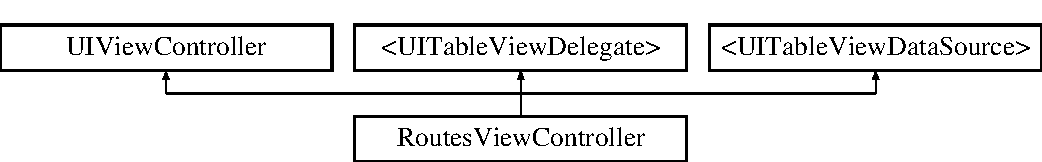
\includegraphics[height=2.000000cm]{interfaceRoutesViewController}
\end{center}
\end{figure}


The documentation for this class was generated from the following file\-:\begin{DoxyCompactItemize}
\item 
In\-Pace/\-In\-Pace/Routes\-View\-Controller.\-h\end{DoxyCompactItemize}

\hypertarget{categoryRoutesViewController_07_08}{\section{Routes\-View\-Controller() Category Reference}
\label{categoryRoutesViewController_07_08}\index{Routes\-View\-Controller()@{Routes\-View\-Controller()}}
}
Inheritance diagram for Routes\-View\-Controller()\-:\begin{figure}[H]
\begin{center}
\leavevmode
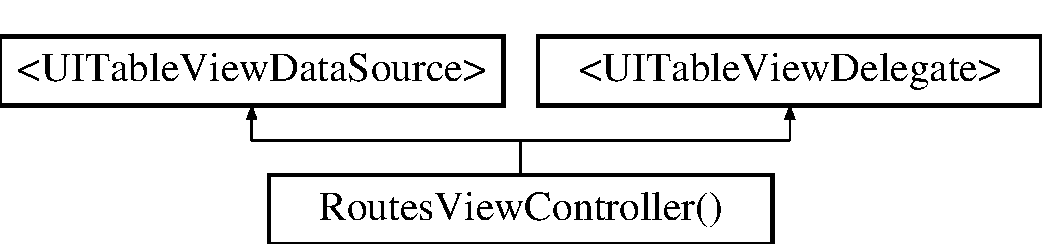
\includegraphics[height=2.000000cm]{categoryRoutesViewController_07_08}
\end{center}
\end{figure}
\subsection*{Instance Methods}
\begin{DoxyCompactItemize}
\item 
(void) -\/ \hyperlink{categoryRoutesViewController_07_08_a645f0e489813bf4b9157d99fbe8f6b61}{load\-Data}
\end{DoxyCompactItemize}
\subsection*{Properties}
\begin{DoxyCompactItemize}
\item 
I\-B\-Outlet U\-I\-Table\-View $\ast$ \hyperlink{categoryRoutesViewController_07_08_a07af2b2999a6ccab5e6941b36b22da85}{tbl\-Routes}
\item 
\hyperlink{interfaceDatabase}{Database} $\ast$ \hyperlink{categoryRoutesViewController_07_08_ae146a192b91c7b6f022ee584d49ef4ec}{db\-Manager}
\item 
N\-S\-Mutable\-Array $\ast$ \hyperlink{categoryRoutesViewController_07_08_a87cf4ac6cc3760cb461ca9461e39664a}{arr\-Routes\-Info}
\item 
long long int \hyperlink{categoryRoutesViewController_07_08_a396bf5c25f2fa8ba025e328758148312}{route\-I\-D}
\end{DoxyCompactItemize}


\subsection{Detailed Description}
\hyperlink{interfaceViewController}{View\-Controller} for viewing all routes in a tableview, option to click on route and view more info 

\subsection{Method Documentation}
\hypertarget{categoryRoutesViewController_07_08_a645f0e489813bf4b9157d99fbe8f6b61}{\index{Routes\-View\-Controller()@{Routes\-View\-Controller()}!load\-Data@{load\-Data}}
\index{load\-Data@{load\-Data}!RoutesViewController()@{Routes\-View\-Controller()}}
\subsubsection[{load\-Data}]{\setlength{\rightskip}{0pt plus 5cm}-\/ (void) load\-Data 
\begin{DoxyParamCaption}
{}
\end{DoxyParamCaption}
}}\label{categoryRoutesViewController_07_08_a645f0e489813bf4b9157d99fbe8f6b61}
Method for loading data from database and putting it into the tableview 

\subsection{Property Documentation}
\hypertarget{categoryRoutesViewController_07_08_a87cf4ac6cc3760cb461ca9461e39664a}{\index{Routes\-View\-Controller()@{Routes\-View\-Controller()}!arr\-Routes\-Info@{arr\-Routes\-Info}}
\index{arr\-Routes\-Info@{arr\-Routes\-Info}!RoutesViewController()@{Routes\-View\-Controller()}}
\subsubsection[{arr\-Routes\-Info}]{\setlength{\rightskip}{0pt plus 5cm}-\/ (N\-S\-Mutable\-Array$\ast$) arr\-Routes\-Info\hspace{0.3cm}{\ttfamily [read]}, {\ttfamily [write]}, {\ttfamily [nonatomic]}, {\ttfamily [strong]}}}\label{categoryRoutesViewController_07_08_a87cf4ac6cc3760cb461ca9461e39664a}
array for holding info of all routes in D\-B \hypertarget{categoryRoutesViewController_07_08_ae146a192b91c7b6f022ee584d49ef4ec}{\index{Routes\-View\-Controller()@{Routes\-View\-Controller()}!db\-Manager@{db\-Manager}}
\index{db\-Manager@{db\-Manager}!RoutesViewController()@{Routes\-View\-Controller()}}
\subsubsection[{db\-Manager}]{\setlength{\rightskip}{0pt plus 5cm}-\/ ({\bf Database}$\ast$) db\-Manager\hspace{0.3cm}{\ttfamily [read]}, {\ttfamily [write]}, {\ttfamily [nonatomic]}, {\ttfamily [strong]}}}\label{categoryRoutesViewController_07_08_ae146a192b91c7b6f022ee584d49ef4ec}
instance of database \hypertarget{categoryRoutesViewController_07_08_a396bf5c25f2fa8ba025e328758148312}{\index{Routes\-View\-Controller()@{Routes\-View\-Controller()}!route\-I\-D@{route\-I\-D}}
\index{route\-I\-D@{route\-I\-D}!RoutesViewController()@{Routes\-View\-Controller()}}
\subsubsection[{route\-I\-D}]{\setlength{\rightskip}{0pt plus 5cm}-\/ (long long int) route\-I\-D\hspace{0.3cm}{\ttfamily [read]}, {\ttfamily [write]}, {\ttfamily [nonatomic]}, {\ttfamily [assign]}}}\label{categoryRoutesViewController_07_08_a396bf5c25f2fa8ba025e328758148312}
holds I\-D of current route \hypertarget{categoryRoutesViewController_07_08_a07af2b2999a6ccab5e6941b36b22da85}{\index{Routes\-View\-Controller()@{Routes\-View\-Controller()}!tbl\-Routes@{tbl\-Routes}}
\index{tbl\-Routes@{tbl\-Routes}!RoutesViewController()@{Routes\-View\-Controller()}}
\subsubsection[{tbl\-Routes}]{\setlength{\rightskip}{0pt plus 5cm}-\/ (I\-B\-Outlet U\-I\-Table\-View$\ast$) tbl\-Routes\hspace{0.3cm}{\ttfamily [read]}, {\ttfamily [write]}, {\ttfamily [nonatomic]}, {\ttfamily [weak]}}}\label{categoryRoutesViewController_07_08_a07af2b2999a6ccab5e6941b36b22da85}
table view 

The documentation for this category was generated from the following file\-:\begin{DoxyCompactItemize}
\item 
In\-Pace/\-In\-Pace/Routes\-View\-Controller.\-m\end{DoxyCompactItemize}

\hypertarget{interfaceSettingsViewController}{\section{Settings\-View\-Controller Class Reference}
\label{interfaceSettingsViewController}\index{Settings\-View\-Controller@{Settings\-View\-Controller}}
}
Inheritance diagram for Settings\-View\-Controller\-:\begin{figure}[H]
\begin{center}
\leavevmode
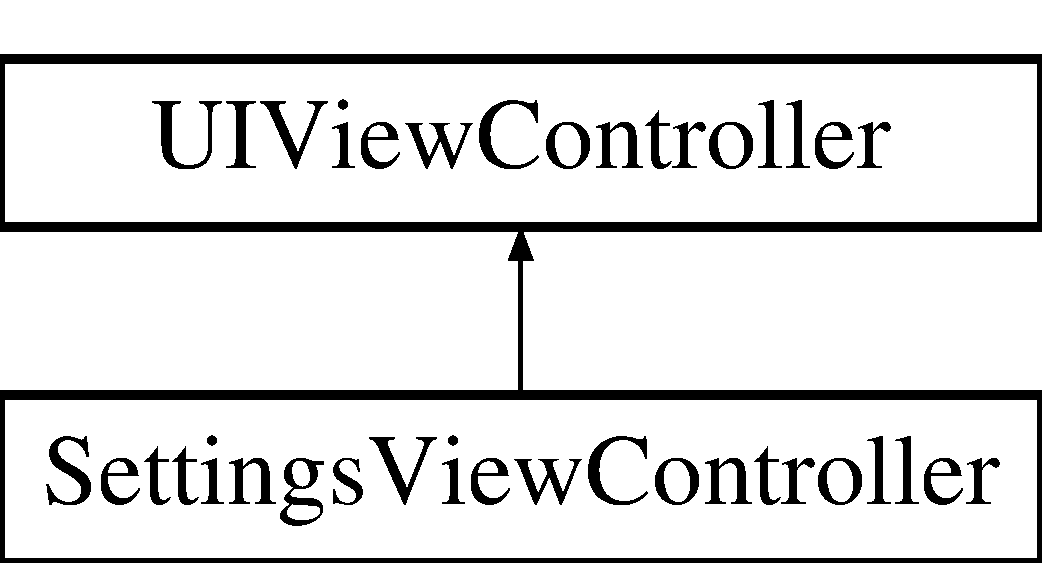
\includegraphics[height=2.000000cm]{interfaceSettingsViewController}
\end{center}
\end{figure}


The documentation for this class was generated from the following file\-:\begin{DoxyCompactItemize}
\item 
In\-Pace/\-In\-Pace/Settings\-View\-Controller.\-h\end{DoxyCompactItemize}

\hypertarget{categorySettingsViewController_07_08}{\section{Settings\-View\-Controller() Category Reference}
\label{categorySettingsViewController_07_08}\index{Settings\-View\-Controller()@{Settings\-View\-Controller()}}
}


The documentation for this category was generated from the following file\-:\begin{DoxyCompactItemize}
\item 
In\-Pace/\-In\-Pace/Settings\-View\-Controller.\-m\end{DoxyCompactItemize}

\hypertarget{interfaceSyncDataViewController}{\section{Sync\-Data\-View\-Controller Class Reference}
\label{interfaceSyncDataViewController}\index{Sync\-Data\-View\-Controller@{Sync\-Data\-View\-Controller}}
}
Inheritance diagram for Sync\-Data\-View\-Controller\-:\begin{figure}[H]
\begin{center}
\leavevmode
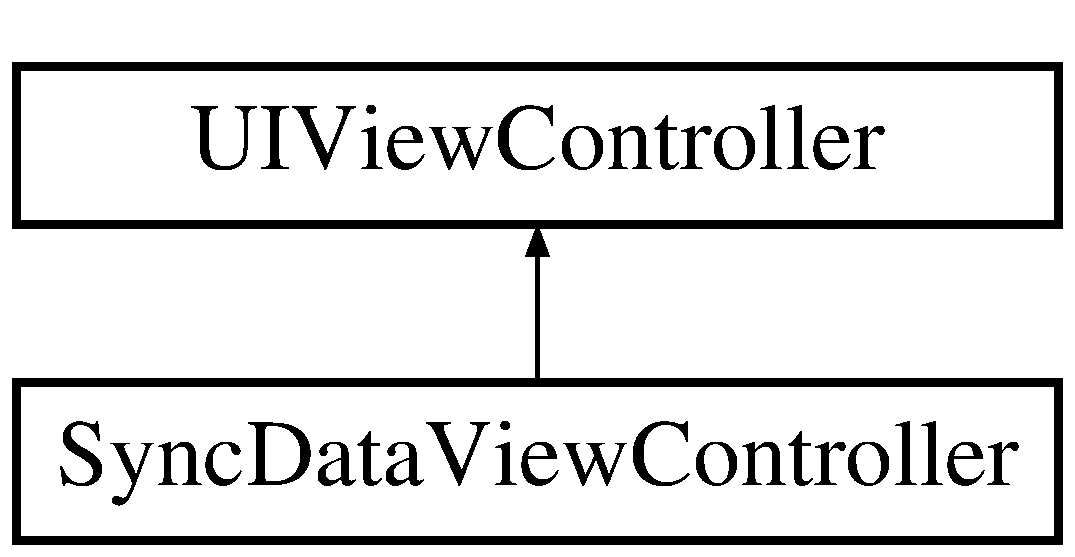
\includegraphics[height=2.000000cm]{interfaceSyncDataViewController}
\end{center}
\end{figure}


The documentation for this class was generated from the following file\-:\begin{DoxyCompactItemize}
\item 
In\-Pace/\-In\-Pace/Sync\-Data\-View\-Controller.\-h\end{DoxyCompactItemize}

\hypertarget{categorySyncDataViewController_07_08}{\section{Sync\-Data\-View\-Controller() Category Reference}
\label{categorySyncDataViewController_07_08}\index{Sync\-Data\-View\-Controller()@{Sync\-Data\-View\-Controller()}}
}
\subsection*{Properties}
\begin{DoxyCompactItemize}
\item 
I\-B\-Outlet U\-I\-Text\-View $\ast$ \hyperlink{categorySyncDataViewController_07_08_a1906b00e4feb73b83bc17f027f8c2bb5}{test\-Text\-View}
\item 
\hyperlink{interfaceBTDiscover}{B\-T\-Discover} $\ast$ \hyperlink{categorySyncDataViewController_07_08_a6c275b0707fdbdb6734f68f3e9e589d0}{discover}
\end{DoxyCompactItemize}


\subsection{Detailed Description}
Sync\-Data\-View\-Controller.\-m\-View\-Controller for showing bluetooth data after syncing 

\subsection{Property Documentation}
\hypertarget{categorySyncDataViewController_07_08_a6c275b0707fdbdb6734f68f3e9e589d0}{\index{Sync\-Data\-View\-Controller()@{Sync\-Data\-View\-Controller()}!discover@{discover}}
\index{discover@{discover}!SyncDataViewController()@{Sync\-Data\-View\-Controller()}}
\subsubsection[{discover}]{\setlength{\rightskip}{0pt plus 5cm}-\/ ({\bf B\-T\-Discover}$\ast$) discover\hspace{0.3cm}{\ttfamily [read]}, {\ttfamily [write]}, {\ttfamily [atomic]}, {\ttfamily [strong]}}}\label{categorySyncDataViewController_07_08_a6c275b0707fdbdb6734f68f3e9e589d0}
instance of \hyperlink{interfaceBTDiscover}{B\-T\-Discover}, to discover peripherals \hypertarget{categorySyncDataViewController_07_08_a1906b00e4feb73b83bc17f027f8c2bb5}{\index{Sync\-Data\-View\-Controller()@{Sync\-Data\-View\-Controller()}!test\-Text\-View@{test\-Text\-View}}
\index{test\-Text\-View@{test\-Text\-View}!SyncDataViewController()@{Sync\-Data\-View\-Controller()}}
\subsubsection[{test\-Text\-View}]{\setlength{\rightskip}{0pt plus 5cm}-\/ (I\-B\-Outlet U\-I\-Text\-View$\ast$) test\-Text\-View\hspace{0.3cm}{\ttfamily [read]}, {\ttfamily [write]}, {\ttfamily [nonatomic]}, {\ttfamily [weak]}}}\label{categorySyncDataViewController_07_08_a1906b00e4feb73b83bc17f027f8c2bb5}
textview for showing data 

The documentation for this category was generated from the following file\-:\begin{DoxyCompactItemize}
\item 
In\-Pace/\-In\-Pace/Sync\-Data\-View\-Controller.\-m\end{DoxyCompactItemize}

\hypertarget{interfaceViewController}{\section{View\-Controller Class Reference}
\label{interfaceViewController}\index{View\-Controller@{View\-Controller}}
}
Inheritance diagram for View\-Controller\-:\begin{figure}[H]
\begin{center}
\leavevmode
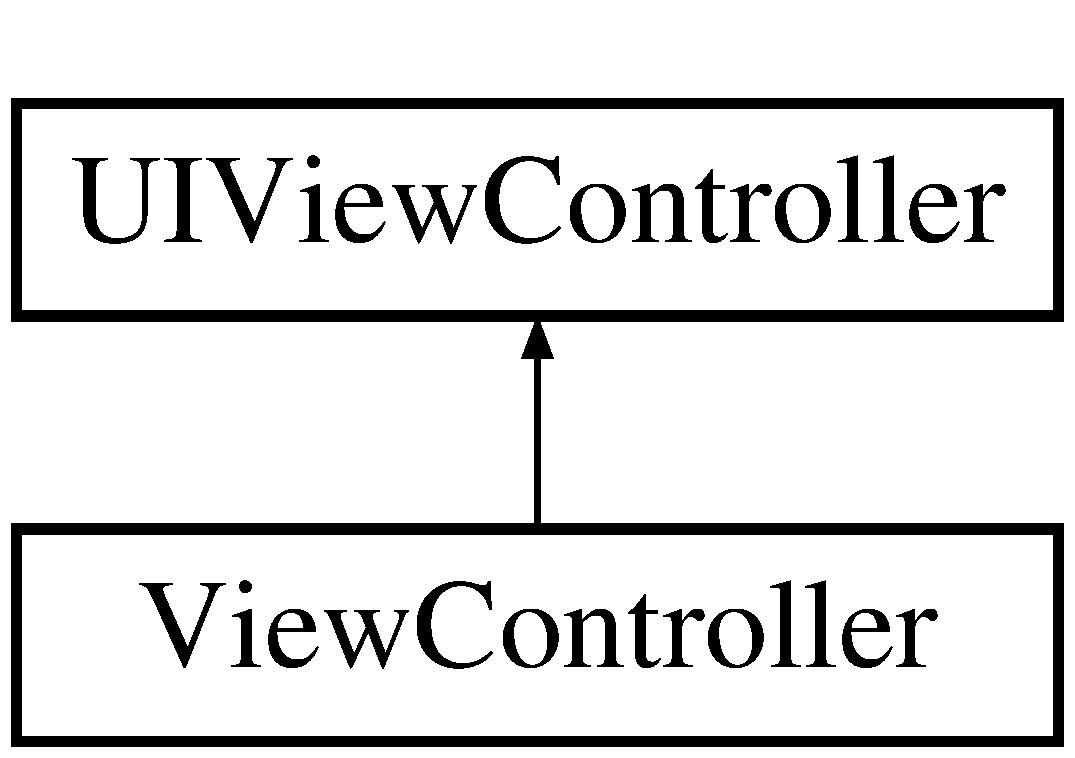
\includegraphics[height=2.000000cm]{interfaceViewController}
\end{center}
\end{figure}


The documentation for this class was generated from the following file\-:\begin{DoxyCompactItemize}
\item 
In\-Pace/\-In\-Pace/View\-Controller.\-h\end{DoxyCompactItemize}

\hypertarget{categoryViewController_07_08}{\section{View\-Controller() Category Reference}
\label{categoryViewController_07_08}\index{View\-Controller()@{View\-Controller()}}
}


\subsection{Detailed Description}
\hyperlink{interfaceViewController}{View\-Controller} for home page 

The documentation for this category was generated from the following file\-:\begin{DoxyCompactItemize}
\item 
In\-Pace/\-In\-Pace/View\-Controller.\-m\end{DoxyCompactItemize}

\chapter{File Documentation}
\hypertarget{BTSendRec_8h}{\section{In\-Pace/\-In\-Pace/\-B\-T\-Send\-Rec.h File Reference}
\label{BTSendRec_8h}\index{In\-Pace/\-In\-Pace/\-B\-T\-Send\-Rec.\-h@{In\-Pace/\-In\-Pace/\-B\-T\-Send\-Rec.\-h}}
}


Bluetooth send and receive functionality.  


{\ttfamily \#import $<$Foundation/\-Foundation.\-h$>$}\\*
{\ttfamily \#import $<$Core\-Bluetooth/\-Core\-Bluetooth.\-h$>$}\\*
{\ttfamily \#import $<$math.\-h$>$}\\*
{\ttfamily \#import $<$time.\-h$>$}\\*
{\ttfamily \#import \char`\"{}Database.\-h\char`\"{}}\\*
\subsection*{Classes}
\begin{DoxyCompactItemize}
\item 
class \hyperlink{interfaceBTSendRec}{B\-T\-Send\-Rec}
\begin{DoxyCompactList}\small\item\em Class responsible for doing the data transmission to the connected peripheral. \end{DoxyCompactList}\end{DoxyCompactItemize}
\subsection*{Macros}
\begin{DoxyCompactItemize}
\item 
\#define \hyperlink{BTSendRec_8h_a417aa5bd52938209ee4c5d2b466183d2}{B\-L\-E\-\_\-\-U\-U\-I\-D}~\mbox{[}C\-B\-U\-U\-I\-D U\-U\-I\-D\-With\-String\-: @\char`\"{}713\-D0000-\/503\-E-\/4\-C75-\/\-B\-A94-\/3148\-F18\-D941\-E\char`\"{}\mbox{]}
\item 
\#define \hyperlink{BTSendRec_8h_a15354b2936317318e52140422b3855af}{R\-X\-\_\-\-U\-U\-I\-D}~\mbox{[}C\-B\-U\-U\-I\-D U\-U\-I\-D\-With\-String\-: @\char`\"{}713\-D0002-\/503\-E-\/4\-C75-\/\-B\-A94-\/3148\-F18\-D941\-E\char`\"{}\mbox{]}
\item 
\#define \hyperlink{BTSendRec_8h_a7badd17f838611be1c30ab64f996735d}{T\-X\-\_\-\-U\-U\-I\-D}~\mbox{[}C\-B\-U\-U\-I\-D U\-U\-I\-D\-With\-String\-: @\char`\"{}713\-D0003-\/503\-E-\/4\-C75-\/\-B\-A94-\/3148\-F18\-D941\-E\char`\"{}\mbox{]}
\item 
\#define \hyperlink{BTSendRec_8h_a85902bfad7a3c74def78040664cad6df}{R\-W\-T\-\_\-\-B\-L\-E\-\_\-\-S\-E\-R\-V\-I\-C\-E\-\_\-\-C\-H\-A\-N\-G\-E\-D\-\_\-\-S\-T\-A\-T\-U\-S\-\_\-\-N\-O\-T\-I\-F\-I\-C\-A\-T\-I\-O\-N}~@\char`\"{}stuff goes here\char`\"{}
\item 
\#define \hyperlink{BTSendRec_8h_aa4f8ea40228c3c3a9a7143b1d1ad8956}{R\-A\-D\-I\-U\-S}~6371000
\item 
\#define \hyperlink{BTSendRec_8h_a598a3330b3c21701223ee0ca14316eca}{P\-I}~3.\-1415926
\item 
\#define \hyperlink{BTSendRec_8h_aeb6c724b0fa46d2ec6ab99cf77f2edd9}{to\-\_\-rad}(x)~((double) x $\ast$ \hyperlink{BTSendRec_8h_a598a3330b3c21701223ee0ca14316eca}{P\-I} / 180)
\end{DoxyCompactItemize}


\subsection{Detailed Description}
Bluetooth send and receive functionality. This file defines the necessary functions and macros to handle reading data from the In\-Pace wristband, parsing it, submitting it to the database, reading values out of the database, and sending the necessary data to the wristband. 

\subsection{Macro Definition Documentation}
\hypertarget{BTSendRec_8h_a417aa5bd52938209ee4c5d2b466183d2}{\index{B\-T\-Send\-Rec.\-h@{B\-T\-Send\-Rec.\-h}!B\-L\-E\-\_\-\-U\-U\-I\-D@{B\-L\-E\-\_\-\-U\-U\-I\-D}}
\index{B\-L\-E\-\_\-\-U\-U\-I\-D@{B\-L\-E\-\_\-\-U\-U\-I\-D}!BTSendRec.h@{B\-T\-Send\-Rec.\-h}}
\subsubsection[{B\-L\-E\-\_\-\-U\-U\-I\-D}]{\setlength{\rightskip}{0pt plus 5cm}\#define B\-L\-E\-\_\-\-U\-U\-I\-D~\mbox{[}C\-B\-U\-U\-I\-D U\-U\-I\-D\-With\-String\-: @\char`\"{}713\-D0000-\/503\-E-\/4\-C75-\/\-B\-A94-\/3148\-F18\-D941\-E\char`\"{}\mbox{]}}}\label{BTSendRec_8h_a417aa5bd52938209ee4c5d2b466183d2}
This macro expands to a C\-B\-U\-U\-I\-D object that represents the U\-U\-I\-D of the Bluetooth shield used in the In\-Pace wristband. \hypertarget{BTSendRec_8h_a598a3330b3c21701223ee0ca14316eca}{\index{B\-T\-Send\-Rec.\-h@{B\-T\-Send\-Rec.\-h}!P\-I@{P\-I}}
\index{P\-I@{P\-I}!BTSendRec.h@{B\-T\-Send\-Rec.\-h}}
\subsubsection[{P\-I}]{\setlength{\rightskip}{0pt plus 5cm}\#define P\-I~3.\-1415926}}\label{BTSendRec_8h_a598a3330b3c21701223ee0ca14316eca}
This macro expands to the value of pi. \hypertarget{BTSendRec_8h_aa4f8ea40228c3c3a9a7143b1d1ad8956}{\index{B\-T\-Send\-Rec.\-h@{B\-T\-Send\-Rec.\-h}!R\-A\-D\-I\-U\-S@{R\-A\-D\-I\-U\-S}}
\index{R\-A\-D\-I\-U\-S@{R\-A\-D\-I\-U\-S}!BTSendRec.h@{B\-T\-Send\-Rec.\-h}}
\subsubsection[{R\-A\-D\-I\-U\-S}]{\setlength{\rightskip}{0pt plus 5cm}\#define R\-A\-D\-I\-U\-S~6371000}}\label{BTSendRec_8h_aa4f8ea40228c3c3a9a7143b1d1ad8956}
This macro expands to the mean radius of the Earth in meters. \hypertarget{BTSendRec_8h_a85902bfad7a3c74def78040664cad6df}{\index{B\-T\-Send\-Rec.\-h@{B\-T\-Send\-Rec.\-h}!R\-W\-T\-\_\-\-B\-L\-E\-\_\-\-S\-E\-R\-V\-I\-C\-E\-\_\-\-C\-H\-A\-N\-G\-E\-D\-\_\-\-S\-T\-A\-T\-U\-S\-\_\-\-N\-O\-T\-I\-F\-I\-C\-A\-T\-I\-O\-N@{R\-W\-T\-\_\-\-B\-L\-E\-\_\-\-S\-E\-R\-V\-I\-C\-E\-\_\-\-C\-H\-A\-N\-G\-E\-D\-\_\-\-S\-T\-A\-T\-U\-S\-\_\-\-N\-O\-T\-I\-F\-I\-C\-A\-T\-I\-O\-N}}
\index{R\-W\-T\-\_\-\-B\-L\-E\-\_\-\-S\-E\-R\-V\-I\-C\-E\-\_\-\-C\-H\-A\-N\-G\-E\-D\-\_\-\-S\-T\-A\-T\-U\-S\-\_\-\-N\-O\-T\-I\-F\-I\-C\-A\-T\-I\-O\-N@{R\-W\-T\-\_\-\-B\-L\-E\-\_\-\-S\-E\-R\-V\-I\-C\-E\-\_\-\-C\-H\-A\-N\-G\-E\-D\-\_\-\-S\-T\-A\-T\-U\-S\-\_\-\-N\-O\-T\-I\-F\-I\-C\-A\-T\-I\-O\-N}!BTSendRec.h@{B\-T\-Send\-Rec.\-h}}
\subsubsection[{R\-W\-T\-\_\-\-B\-L\-E\-\_\-\-S\-E\-R\-V\-I\-C\-E\-\_\-\-C\-H\-A\-N\-G\-E\-D\-\_\-\-S\-T\-A\-T\-U\-S\-\_\-\-N\-O\-T\-I\-F\-I\-C\-A\-T\-I\-O\-N}]{\setlength{\rightskip}{0pt plus 5cm}\#define R\-W\-T\-\_\-\-B\-L\-E\-\_\-\-S\-E\-R\-V\-I\-C\-E\-\_\-\-C\-H\-A\-N\-G\-E\-D\-\_\-\-S\-T\-A\-T\-U\-S\-\_\-\-N\-O\-T\-I\-F\-I\-C\-A\-T\-I\-O\-N~@\char`\"{}stuff goes here\char`\"{}}}\label{BTSendRec_8h_a85902bfad7a3c74def78040664cad6df}
No idea what this does or why it's here, honestly... \hypertarget{BTSendRec_8h_a15354b2936317318e52140422b3855af}{\index{B\-T\-Send\-Rec.\-h@{B\-T\-Send\-Rec.\-h}!R\-X\-\_\-\-U\-U\-I\-D@{R\-X\-\_\-\-U\-U\-I\-D}}
\index{R\-X\-\_\-\-U\-U\-I\-D@{R\-X\-\_\-\-U\-U\-I\-D}!BTSendRec.h@{B\-T\-Send\-Rec.\-h}}
\subsubsection[{R\-X\-\_\-\-U\-U\-I\-D}]{\setlength{\rightskip}{0pt plus 5cm}\#define R\-X\-\_\-\-U\-U\-I\-D~\mbox{[}C\-B\-U\-U\-I\-D U\-U\-I\-D\-With\-String\-: @\char`\"{}713\-D0002-\/503\-E-\/4\-C75-\/\-B\-A94-\/3148\-F18\-D941\-E\char`\"{}\mbox{]}}}\label{BTSendRec_8h_a15354b2936317318e52140422b3855af}
This macro expands to a C\-B\-U\-U\-I\-D object that represents the U\-U\-I\-D of the Read characteristic on the Bluetooth shield. \hypertarget{BTSendRec_8h_aeb6c724b0fa46d2ec6ab99cf77f2edd9}{\index{B\-T\-Send\-Rec.\-h@{B\-T\-Send\-Rec.\-h}!to\-\_\-rad@{to\-\_\-rad}}
\index{to\-\_\-rad@{to\-\_\-rad}!BTSendRec.h@{B\-T\-Send\-Rec.\-h}}
\subsubsection[{to\-\_\-rad}]{\setlength{\rightskip}{0pt plus 5cm}\#define to\-\_\-rad(
\begin{DoxyParamCaption}
\item[{}]{x}
\end{DoxyParamCaption}
)~((double) x $\ast$ {\bf P\-I} / 180)}}\label{BTSendRec_8h_aeb6c724b0fa46d2ec6ab99cf77f2edd9}
This macro takes the value x and converts it into radians. \hypertarget{BTSendRec_8h_a7badd17f838611be1c30ab64f996735d}{\index{B\-T\-Send\-Rec.\-h@{B\-T\-Send\-Rec.\-h}!T\-X\-\_\-\-U\-U\-I\-D@{T\-X\-\_\-\-U\-U\-I\-D}}
\index{T\-X\-\_\-\-U\-U\-I\-D@{T\-X\-\_\-\-U\-U\-I\-D}!BTSendRec.h@{B\-T\-Send\-Rec.\-h}}
\subsubsection[{T\-X\-\_\-\-U\-U\-I\-D}]{\setlength{\rightskip}{0pt plus 5cm}\#define T\-X\-\_\-\-U\-U\-I\-D~\mbox{[}C\-B\-U\-U\-I\-D U\-U\-I\-D\-With\-String\-: @\char`\"{}713\-D0003-\/503\-E-\/4\-C75-\/\-B\-A94-\/3148\-F18\-D941\-E\char`\"{}\mbox{]}}}\label{BTSendRec_8h_a7badd17f838611be1c30ab64f996735d}
This macro expands to a C\-B\-U\-U\-I\-D object that represents the U\-U\-I\-D of the Write characteristic on the Bluetooth shield. 
%--- End generated contents ---

% Index
\newpage
\phantomsection
\addcontentsline{toc}{chapter}{Index}
\printindex

\end{document}
